\documentclass{article}


\usepackage{amsmath}
\usepackage[document]{ragged2e}
\usepackage{listings}
\usepackage{color}
\usepackage[T1]{fontenc} % Use 8-bit encoding that has 256 glyphs
\usepackage{fourier} % Use the Adobe Utopia font for the document - comment this line to return to the LaTeX default
\usepackage[english]{babel} % English language/hyphenation
\usepackage{amsmath,amsfonts,amsthm} % Math packages
\usepackage{graphicx}
\usepackage{float}

\numberwithin{equation}{section} % Number equations within sections (i.e. 1.1, 1.2, 2.1, 2.2 instead of 1, 2, 3, 4)

\usepackage{sectsty} % Allows customizing section commands
\allsectionsfont{\centering \normalfont\scshape} % Make all sections centered, the default font and small caps

%
%
%Below is setting style, copied from
%https://www.sharelatex.com/learn/Code_listing
%
%
%
\definecolor{codegreen}{rgb}{0,0.6,0}
\definecolor{codegray}{rgb}{0.5,0.5,0.5}
\definecolor{codepurple}{rgb}{0.58,0,0.82}
\definecolor{backcolour}{rgb}{0.95,0.95,0.92}

\lstdefinestyle{mystyle}{
	backgroundcolor=\color{backcolour},  
	commentstyle=\color{codegreen},
	keywordstyle=\color{magenta},
	numberstyle=\tiny\color{codegray},
	stringstyle=\color{codepurple},
	basicstyle=\footnotesize,
	breakatwhitespace=false,         
	breaklines=true,                 
	captionpos=b,                    
	keepspaces=true,                 
	numbers=left,                    
	numbersep=5pt,                  
	showspaces=false,                
	showstringspaces=false,
	showtabs=false,                  
	tabsize=2
}

\lstset{style=mystyle}

%----------------------------------------------------------------------------------------
%	TITLE SECTION
%----------------------------------------------------------------------------------------

\newcommand{\horrule}[1]{\rule{\linewidth}{#1}} % Create horizontal rule command with 1 argument of height


\begin{document}
	\begin{titlepage}
		\centering
		{\LARGE\bfseries } \par
		\vspace{5mm}
		{\huge Incomplete Data Analysis Assignment (5\%)}\par
		\vspace{5mm}
		\large{S1889112}
	\end{titlepage}
	\newpage	
	

\subsection*{a) (10 marks)} 

\textbf{Carry out a CCA to find the mean value of the recovery time (and associated standard error) and to find also the correlations between the recovery time and the dose and between the recovery time and blood pressure.}

\vspace{5mm}

A complete case analysis means dropping any missing data from the dataset, and then calculating our summary statistics. \\

Using a complete case analysis, the mean value of recovery time is 19.272, with an associated standard error of 2.442. The correlation between recovery time and the dose is 0.238, while the correlation between recovery time and blood pressure is -0.020. All results are to 3 decimal places. 


\subsection*{b) (15 marks)} 

\textbf{The same as in (a) but using mean imputation}

\vspace{5mm}

Mean imputation takes the complete case mean, and uses this in place of the missing values. \\

Using mean imputation, the mean value of recovery time is unchanged at 19.272, but with an associated standard error of 2.284. The correlation between recovery time and the dose is 0.215, while the correlation between recovery time and blood pressure is -0.019. All results are to 3 decimal places. 

\subsection*{c) (15 marks)} 

\textbf{The same as in (a) but using mean regression imputation}

\vspace{5mm}

Regression imputation takes the complete cases, performs linear regression (with our missing column as the response), and then uses the predictions E(Y|X) in place of the missing data.  \\

Using regression imputation, the mean value of recovery time is 19.444, with an associated standard error of 2.313. The correlation between recovery time and the dose is 0.279, while the correlation between recovery time and blood pressure is -0.011. All results are to 3 decimal places. 

\newpage
\subsection*{d) (15 marks)} 

\textbf{The same as in (a) but using stochastic regression imputation. Do you need any extra care when conducting stochastic regression imputation in this example?}

\vspace{5mm}
Stochastic regression imputation is identical to regression imputation but with an extra step. This involves adding 
noise to the predictions to try and restore lost variability from only using regression imputation. We assume the error is distributed normally with a mean of 0, and a homoscedastic variance equal to the estimated variance of the residuals from the complete case regression.
\\
Using stochastic regression imputation, the mean value of recovery time is 19.903, with an associated standard error of 2.337. The correlation between recovery time and the dose is 0.295, while the correlation between recovery time and blood pressure is -0.0013. All results are to 3 decimal places. 
\\
Figure 1 shows the residual quantiles plotted against the quantiles for a normal curve (a qq plot). It shows that the sample quantiles for the residuals are consistently above the normal quantiles (illustrated by the lines). This suggests the residuals are not normally distributed, hence generating a normal error for the predictions is invalid. 
\\
%
%
% [H] option from float package
% ensures figure stays in place
%
\begin{figure}[H]
	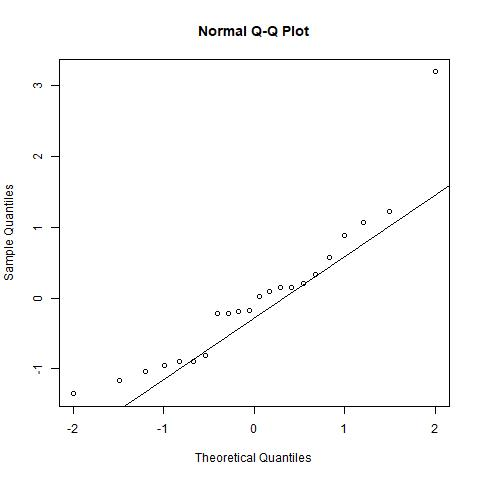
\includegraphics[scale=0.60]{qqplot.jpg}
	\caption{QQ plot}
\end{figure}
\newpage
\subsection*{e) (30 marks)}
\textbf{You will now conduct the same analysis but applying another technique called predictive mean matching (Little, 1988), which is a special type of hot deck imputation. In the simplest form of this method (and the one you will use here), a regression model is used to predict the variables with missing values from the other (complete) variables. For each subject with a missing value, the donor is chosen to be the subject with a predicted value of her or his own that is closest (to be measured by the squared difference) to the prediction for the subject with the missing value.}


\vspace{5mm}
Hot deck in general attempts to impute values by just using similar individuals instead of creating predictions. In the following example, by nature of linear regression - similar individuals implies similar predictions, and we use these predictions to find the most similar individual, and impute using their value. \\

Using hot deck imputation, the mean value of recovery time is 19.440, with an associated standard error of 2.464. The correlation between recovery time and the dose is 0.314, while the correlation between recovery time and blood pressure is -0.032. All results are to 3 decimal places. 


\subsection*{f) (15 marks)}
\textbf{What is an obvious advantage of predictive mean matching over stochastic regression imputation?}

Predictive mean matching avoids extrapolation beyond the range of values in the dataset, and so predictions based on this methodology are more likely to follow the true distribution. Additionally, it maintains discrete responses. 

\newpage
\appendix
\section{R Code}
\begin{lstlisting}[language=R]
#------------------------------------#
############## PREAMBLE ##############
#------------------------------------# 

load(file = 'databp.Rdata')
databp$missing <- ifelse(databp$R==0, 1, 0)
n <- nrow(databp)


#------------------------------------#
############### PART A ###############
#------------------------------------#

# Create df with only observed data

databp.cca <- databp[databp$missing == 0, ]


# Calculate statistics
mean.cca             <- mean(databp.cca$recovtime)
se.cca               <- sd  (databp.cca$recovtime)/sqrt(n)
cor.recov.dose.cca   <- cor (databp.cca$recovtime, exp(databp.cca$logdose))
cor.recov.bloodp.cca <- cor (databp.cca$recovtime, databp.cca$bloodp )


#### Results Part A ####

c(mean.cca, se.cca, cor.recov.dose.cca, cor.recov.bloodp.cca)



#------------------------------------#
############### PART B ###############
#------------------------------------#

# Already have complete case mean, which is the mean to impute
# Impute into new df
df.MI <- databp
df.MI$recovtime <- ifelse(df.MI$missing == 1, mean.cca, df.MI$recovtime)

# Calculate statistics


mean.MI             <- mean(df.MI$recovtime)
se.MI               <- sd  (df.MI$recovtime)/sqrt(n)
cor.recov.dose.MI   <- cor (df.MI$recovtime, exp(df.MI$logdose))
cor.recov.bloodp.MI <- cor (df.MI$recovtime, df.MI$bloodp)



#### Results Part B ####
c(mean.MI, se.MI, cor.recov.dose.MI, cor.recov.bloodp.MI)



#------------------------------------#
############### PART C ###############
#------------------------------------#

# Create new df
df.RI <- databp


# Fit model (lm ignores missing values), and generate predictions
mod            <- lm(recovtime ~ bloodp + logdose, data = df.RI)
predictions.RI <- predict(mod, df.RI)

# Impute predictions to missing data
# If data missing, use prediction, otherwise use true value
df.RI$recovtime <- ifelse(df.RI$missing==1, predictions.RI, df.RI$recovtime)

# Calculate statistics


mean.RI             <- mean(df.RI$recovtime)
se.RI               <- sd  (df.RI$recovtime)/sqrt(n)
cor.recov.dose.RI   <- cor (df.RI$recovtime, exp(df.RI$logdose))
cor.recov.bloodp.RI <- cor (df.RI$recovtime, df.RI$bloodp)

#### Results Part C ####
c(mean.RI, se.RI, cor.recov.dose.RI, cor.recov.bloodp.RI)


#------------------------------------#
############### PART D ###############
#------------------------------------#
set.seed(36)
# Already have regression results from part C
# Just need to add noise onto predictions

# SRI is just an extension of RI, so use df.RI as basis for new df
# Get noise scale parameter
df.SRI   <- df.RI
noise.sd <- summary(mod)$sigma
# Add normal error if data was missing
df.SRI$recovtime <- ifelse(df.SRI$missing==1, 
                           df.SRI$recovtime + rnorm(1, 0, noise.sd),
                           df.SRI$recovtime)
# Calculate statistics
mean.SRI             <- mean(df.SRI$recovtime)
se.SRI               <- sd  (df.SRI$recovtime)/sqrt(n)
cor.recov.dose.SRI   <- cor (df.SRI$recovtime, exp(df.SRI$logdose))
cor.recov.bloodp.SRI <- cor (df.SRI$recovtime, df.SRI$bloodp)

#### Results Part D ####
c(mean.SRI, se.SRI, cor.recov.dose.SRI, cor.recov.bloodp.SRI)

# Linear regression assumption of normally distributed errors
jpeg('LaTeX/qqplot.jpg')
qqnorm(rstandard(mod))
qqline(rstandard(mod))
dev.off()
#------------------------------------#
############### PART E ###############
#------------------------------------#
# Distance function
distance <- function(x,y) sqrt((x-y)^2)

# New df
df.HD <- databp

# Regression model recycled from RI section
mod.HD <- mod

# Predict for each item in data, and store in the dataframe for validity checks
df.HD$predictions        <- predict.lm(mod.HD, newdata = df.HD)
df.HD$hotdeckpredictions <- numeric(n)

# Loop through rows
for (person in 1:n){
    # If data not missing, just use observed value
  if (df.HD[person, 'R'] == 1) {
    df.HD[person, 'hotdeckpredictions'] <- df.HD[person, 'recovtime']
  } else {
    # Get missing person's predicted value, and calculate distance to
    # all others' predicted value
    predval   <- df.HD[person, 'predictions']
    distances <- distance(predval, df.HD$predictions)
    # Find index of smallest distance that doesn't belong to the current or any 
    # other missing person
    mindist <- min(distances[distances>0 & df.HD$missing==0])
    minindex <- which(distances == mindist)
    # Use that index's true value as the prediction for the missing person
    df.HD[person, 'hotdeckpredictions'] <- df.HD[minindex, 'recovtime']
    # Create min index column for manual inspection of process. 
    df.HD[person, 'minindex'] <- minindex
  }
}

# View(df.HD)
# Sort by predictions in view to see method has used nearest prediction for
# the true value

# Perform imputation
df.HD$recovtime <- df.HD$hotdeckpredictions


# Calculate statistics

mean.HD             <- mean(df.HD$recovtime)
se.HD               <- sd  (df.HD$recovtime)/sqrt(n)
cor.recov.dose.HD   <- cor (df.HD$recovtime, exp(df.HD$logdose))
cor.recov.bloodp.HD <- cor (df.HD$recovtime, df.HD$bloodp)

#### Results Part E ####
c(mean.HD, se.HD, cor.recov.dose.HD, cor.recov.bloodp.HD)


\end{lstlisting}








\end{document}
